\chapter{Analisi dei requisiti}
\label{cap:analisi-requisiti}

\par L'analisi dei \gls{requisiti} è stata condotta seguendo gli standard dell'ingegneria del software, integrando la valutazione delle soluzioni esistenti con colloqui e dialoghi con la Proponente. In questa sezione vengono illustrati i seguenti punti:
\begin{itemize}
    \item \textbf{\Gls{use-case}}: descrizione e diagrammi dei casi d'uso;
    \item \textbf{Tracciamento dei requisiti}: associa ciascun requisito alla sua fonte di provenienza;
    \item \textbf{\Gls{user-story}}: descrizione delle esigenze dell’utente finale.
\end{itemize}

\section{Casi d'uso}

\paragraph*{Attori}
\par L'unico attore coinvolto nell'interazione con il sistema è un \textbf{utente generico} con accesso completo allo strumento di analisi \gls{seo}. Di seguito sono elencate alcune tipologie di utenti a cui è rivolto il progetto:
\begin{itemize}
    \item \textbf{Sviluppatore}: utilizza l'estensione durante lo sviluppo e la produzione di contenuti web;
    \item \textbf{Tester}: effettua un'analisi \gls{seo} per identificare eventuali problemi e proporre azioni di miglioramento;
    \item \textbf{Professore}: utilizza l'estensione per analizzare progetti didattici.
\end{itemize}

\begin{usecase}{1}{Accesso allo strumento di analisi delle parole chiave}\label{UC1}
    \usecaseactors{Utente.}
    \usecasepre{L'utente ha avviato l'estensione.}
    \usecasedesc{L'utente seleziona lo strumento di analisi delle parole chiave.}
    \usecasepost{Il sistema mostra la schermata di analisi delle parole chiave.}
\end{usecase}

\vspace{10pt}
\par\noindent La figura \ref{fig:uc1} illustra graficamente il caso d’uso UC1.

\begin{figure}[H]
  \centering
  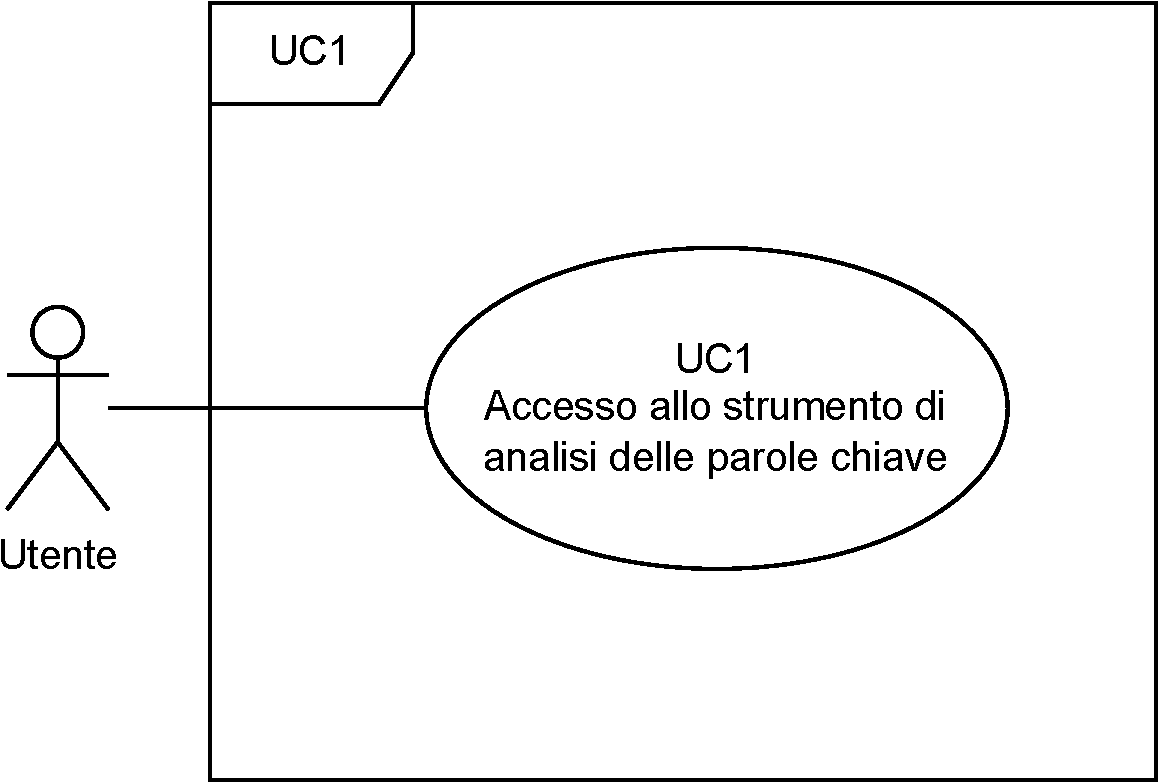
\includegraphics[width=0.6\textwidth]{usecase/uc_1.pdf}
  \caption{UC1}
  \label{fig:uc1}
\end{figure}

\begin{usecase}{2}{Visualizzazione di una panoramica dell'analisi delle parole chiave}\label{UC2}
    \usecaseactors{Utente.}
    \usecasepreEnv{\begin{itemize}
        \item L'utente ha selezionato lo strumento di analisi delle parole chiave;
        \item Il sistema è attivo e funzionante.
    \end{itemize}}
    \usecasepost{Il sistema mostra una panoramica dell'analisi delle parole chiave.}
    \usecasesubEnv{\begin{itemize}
        \item \hyperref[UC2point1]{UC2.1}: Visualizzazione del meta tag keywords;
        \item \hyperref[UC2point2]{UC2.2}: Visualizzazione del numero totale di parole nella pagina;
        \item \hyperref[UC2point3]{UC2.3}: Visualizzazione del numero di parole uniche nella pagina;
        \item \hyperref[UC2point4]{UC2.4}: Visualizzazione della lingua della pagina.
    \end{itemize}}
\end{usecase}

\vspace{10pt}
\par\noindent La figura \ref{fig:uc2} illustra graficamente il caso d’uso UC2.

\begin{figure}[H]
  \centering
  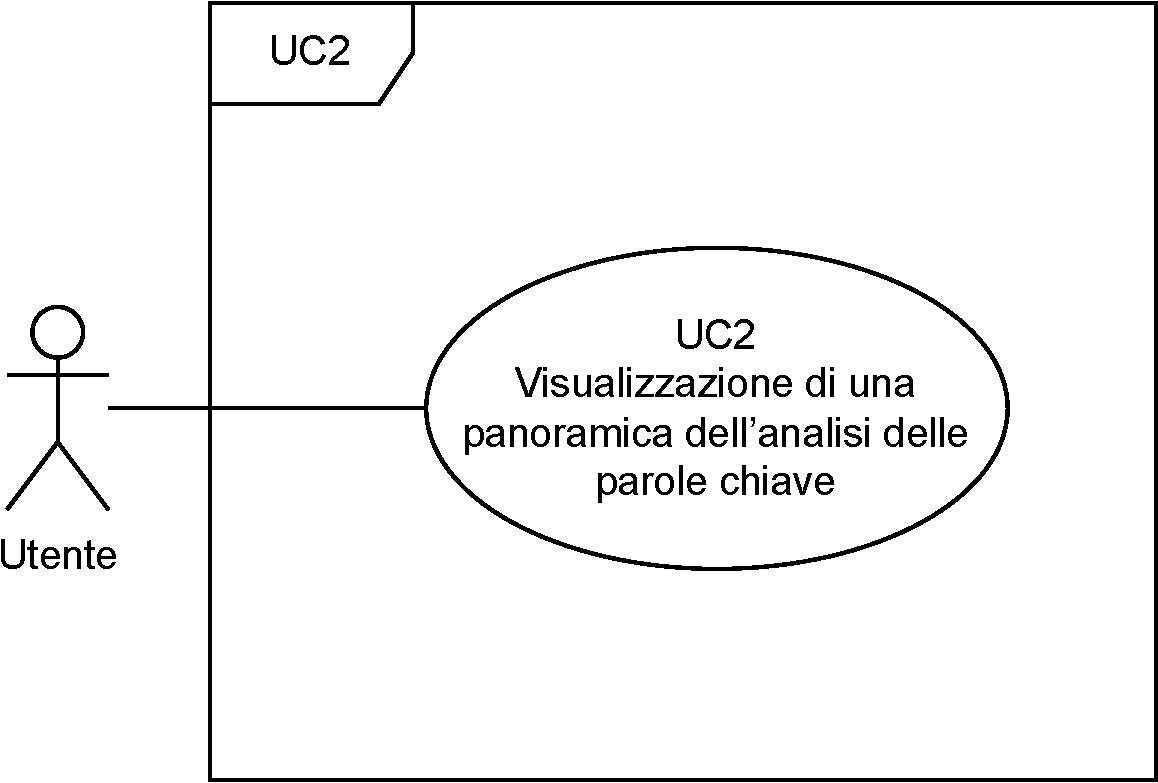
\includegraphics[width=0.6\textwidth]{usecase/uc_2.pdf}
  \caption{UC2}
  \label{fig:uc2}
\end{figure}

\begin{usecase}{2.1}{Visualizzazione del meta tag keywords}\label{UC2point1}
    \usecaseactors{Utente.}
    \usecasepreEnv{\begin{itemize}
        \item L'utente ha selezionato lo strumento di analisi delle parole chiave;
        \item Il sistema è attivo e funzionante.
    \end{itemize}}
    \usecasepost{Il sistema mostra il contenuto del meta tag keywords.}
    \usecaseextEnv{\begin{itemize}
        \item \hyperref[UC19]{UC19}: Visualizzazione di un avviso se il meta tag keywords non è presente.
    \end{itemize}}
\end{usecase}

\begin{usecase}{2.2}{Visualizzazione del numero totale di parole nella pagina}\label{UC2point2}
    \usecaseactors{Utente.}
    \usecasepreEnv{\begin{itemize}
        \item L'utente ha selezionato lo strumento di analisi delle parole chiave;
        \item Il sistema è attivo e funzionante.
    \end{itemize}}
    \usecasepost{Il sistema mostra il numero totale di parole presenti nella pagina.}
\end{usecase}

\begin{usecase}{2.3}{Visualizzazione del numero di parole uniche nella pagina}\label{UC2point3}
    \usecaseactors{Utente.}
    \usecasepreEnv{\begin{itemize}
        \item L'utente ha selezionato lo strumento di analisi delle parole chiave;
        \item Il sistema è attivo e funzionante.
    \end{itemize}}
    \usecasepost{Il sistema mostra il numero di parole uniche presenti nella pagina.}
\end{usecase}

\begin{usecase}{2.4}{Visualizzazione della lingua della pagina}\label{UC2point4}
    \usecaseactors{Utente.}
    \usecasepreEnv{\begin{itemize}
        \item L'utente ha selezionato lo strumento di analisi delle parole chiave;
        \item Il sistema è attivo e funzionante.
    \end{itemize}}
    \usecasepost{Il sistema mostra la lingua dichiarata nella pagina.}
    \usecaseextEnv{\begin{itemize}
        \item \hyperref[UC20]{UC20}: Visualizzazione di un avviso se l'attributo lang non è presente.
    \end{itemize}}
\end{usecase}

\vspace{10pt}
\par\noindent La figura \ref{fig:uc2_sottocasi} illustra graficamente i sottocasi del caso d'uso UC2.

\begin{figure}[H]
  \centering
  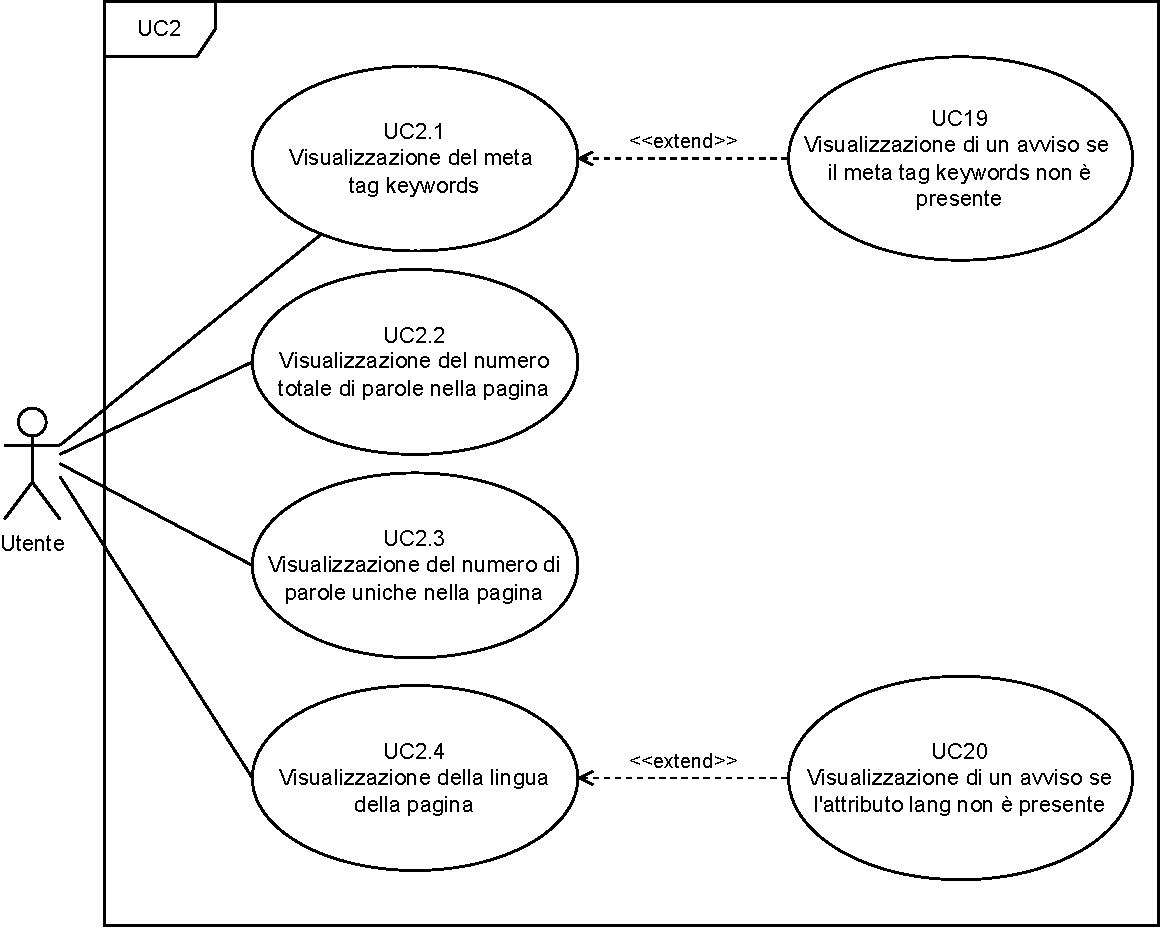
\includegraphics[width=0.95\textwidth]{usecase/uc_2_sottocasi.pdf}
  \caption{UC2 - sottocasi}
  \label{fig:uc2_sottocasi}
\end{figure}

\begin{usecase}{3}{Inserimento di una parola chiave}\label{UC3}
    \usecaseactors{Utente.}
    \usecasepreEnv{\begin{itemize}
        \item L'utente ha selezionato lo strumento di analisi delle parole chiave;
        \item Il sistema è attivo e funzionante.
    \end{itemize}}
    \usecasedesc{L'utente digita una parola chiave.}
    \usecasepost{Il sistema mostra la parola chiave inserita dall'utente nell'apposito campo di testo.}
\end{usecase}

\vspace{10pt}
\par\noindent La figura \ref{fig:uc3} illustra graficamente il caso d'uso UC3.

\begin{figure}[H]
  \centering
  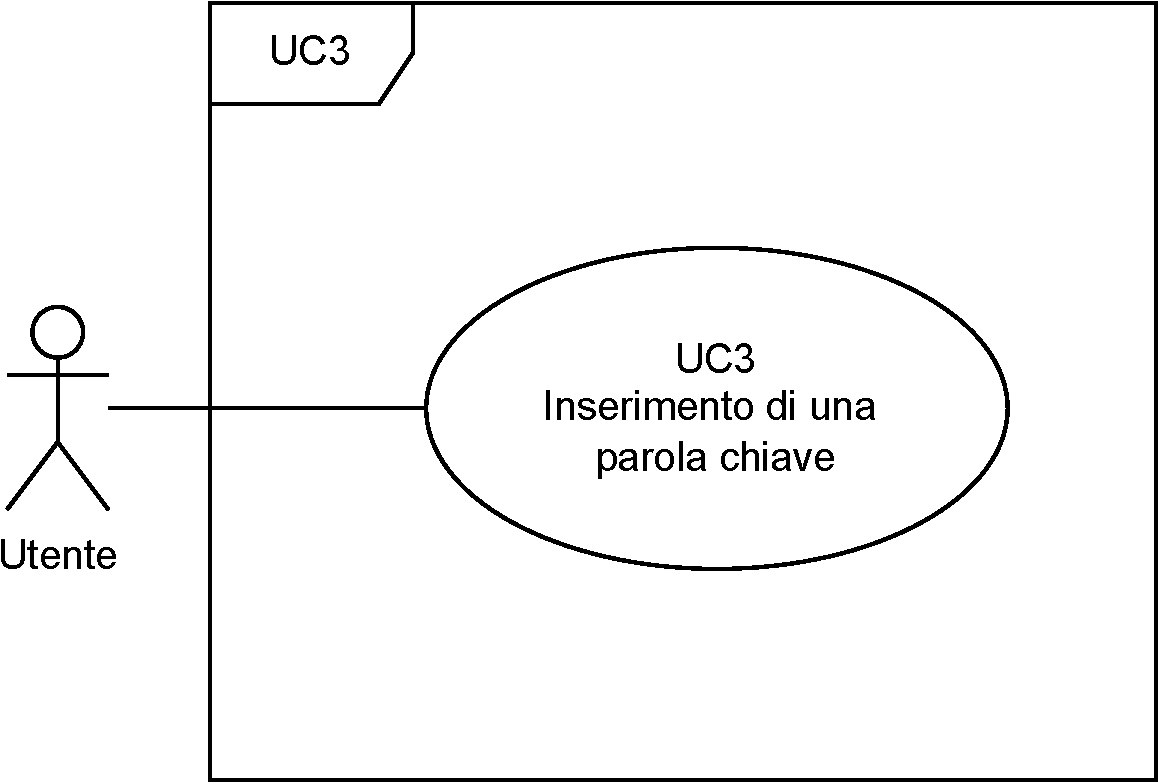
\includegraphics[width=0.6\textwidth]{usecase/uc_3.pdf}
  \caption{UC3}
  \label{fig:uc3}
\end{figure}

\begin{usecase}{4}{Analisi della parola chiave digitata}\label{UC4}
    \usecaseactors{Utente.}
    \usecasepreEnv{\begin{itemize}
        \item L'utente ha selezionato lo strumento di analisi delle parole chiave;
        \item Il sistema è attivo e funzionante;
        \item L'utente ha digitato una parola chiave.
    \end{itemize}}
    \usecasedesc{Il sistema esegue l'analisi della parola chiave digitata dall'utente.}
    \usecasepost{Il sistema aggiunge la parola chiave analizzata alla lista delle keyword.}
    \usecaseincEnv{\begin{itemize}
        \item \hyperref[UC3]{UC3}: Inserimento di una parola chiave.
    \end{itemize}}
\end{usecase}

\vspace{10pt}
\par\noindent La figura \ref{fig:uc4} illustra graficamente il caso d'uso UC4.

\begin{figure}[H]
  \centering
  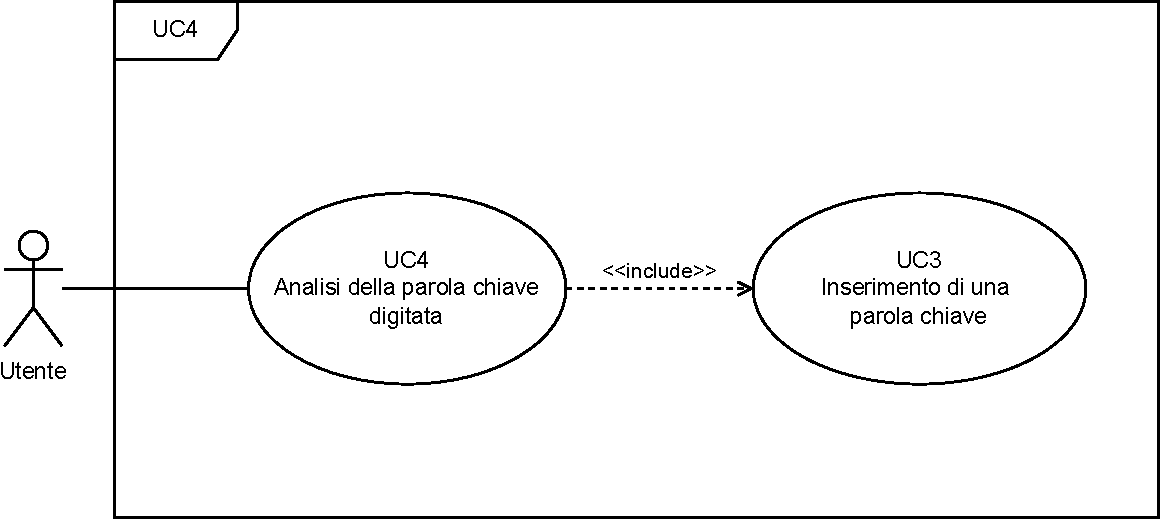
\includegraphics[width=0.95\textwidth]{usecase/uc_4.pdf}
  \caption{UC4}
  \label{fig:uc4}
\end{figure}

\begin{usecase}{5}{Visualizzazione di una lista delle parole chiave}\label{UC5}
    \usecaseactors{Utente.}
    \usecasepreEnv{\begin{itemize}
        \item L'utente ha selezionato lo strumento di analisi delle parole chiave;
        \item Il sistema è attivo e funzionante.
    \end{itemize}}
    \usecasepost{Il sistema mostra una lista delle parole chiave.}
    \usecasesubEnv{\begin{itemize}
        \item \hyperref[UC5point1]{UC5.1}: Visualizzazione di una lista delle parole chiave estratte dal meta tag keywords;
        \item \hyperref[UC5point2]{UC5.2}: Visualizzazione di una lista delle parole chiave inserite dall'utente;
        \item \hyperref[UC5point3]{UC5.3}: Visualizzazione di una lista delle parole chiave più frequenti.
    \end{itemize}}
    \usecaseincEnv{\begin{itemize}
        \item \hyperref[UC6]{UC6}: Visualizzazione di una singola parola chiave all’interno della lista.
    \end{itemize}}
\end{usecase}

\vspace{10pt}
\par\noindent La figura \ref{fig:uc5} illustra graficamente il caso d'uso UC5.

\begin{figure}[H]
  \centering
  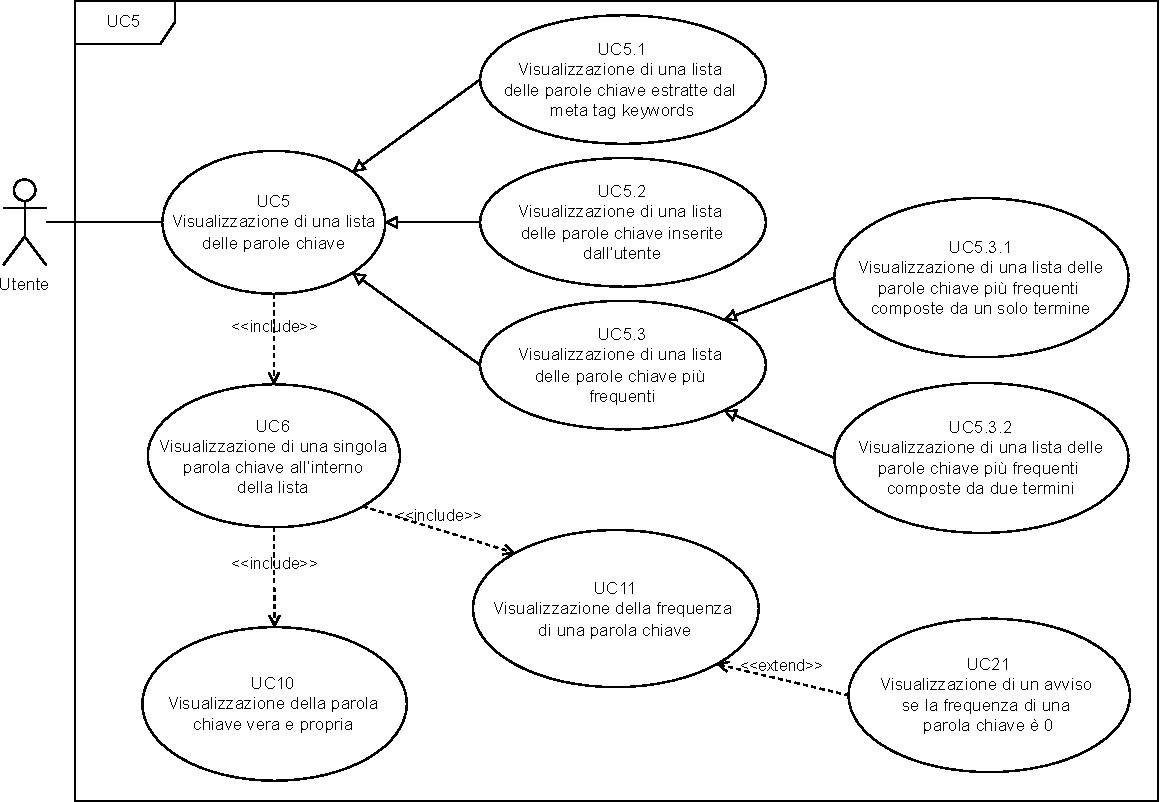
\includegraphics[width=\textwidth]{usecase/uc_5.pdf}
  \caption{UC5}
  \label{fig:uc5}
\end{figure}

\begin{usecase}{5.1}{Visualizzazione di una lista delle parole chiave estratte dal meta tag keywords}\label{UC5point1}
    \usecaseactors{Utente.}
    \usecasepreEnv{\begin{itemize}
        \item L'utente ha selezionato lo strumento di analisi delle parole chiave;
        \item Il sistema è attivo e funzionante.
    \end{itemize}}
    \usecasepost{Il sistema mostra una lista delle parole chiave estratte dal meta tag keywords.}
\end{usecase}

\begin{usecase}{5.2}{Visualizzazione di una lista delle parole chiave inserite dall'utente}\label{UC5point2}
    \usecaseactors{Utente.}
    \usecasepreEnv{\begin{itemize}
        \item L'utente ha selezionato lo strumento di analisi delle parole chiave;
        \item Il sistema è attivo e funzionante.
    \end{itemize}}
    \usecasepost{Il sistema mostra una lista delle parole chiave inserite dall'utente.}
\end{usecase}

\begin{usecase}{5.3}{Visualizzazione di una lista delle parole chiave più frequenti}\label{UC5point3}
    \usecaseactors{Utente.}
    \usecasepreEnv{\begin{itemize}
        \item L'utente ha selezionato lo strumento di analisi delle parole chiave;
        \item Il sistema è attivo e funzionante.
    \end{itemize}}
    \usecasepost{Il sistema mostra una lista delle parole chiave più frequenti, estratte automaticamente da un algoritmo interno.}
    \usecasesubEnv{\begin{itemize}
        \item \hyperref[UC5point3point1]{UC5.3.1}: Visualizzazione di una lista delle parole chiave più frequenti composte da un solo termine;
        \item \hyperref[UC5point3point2]{UC5.3.2}: Visualizzazione di una lista delle parole chiave più frequenti composte da due termini.
    \end{itemize}}
\end{usecase}

\begin{usecase}{5.3.1}{Visualizzazione di una lista delle parole chiave più frequenti composte da un solo termine}\label{UC5point3point1}
    \usecaseactors{Utente.}
    \usecasepreEnv{\begin{itemize}
        \item L'utente ha selezionato lo strumento di analisi delle parole chiave;
        \item Il sistema è attivo e funzionante.
    \end{itemize}}
    \usecasepost{Il sistema mostra una lista delle parole chiave più frequenti composte da un solo termine (keyword semplici).}
\end{usecase}

\begin{usecase}{5.3.2}{Visualizzazione di una lista delle parole chiave più frequenti composte da due termini}\label{UC5point3point2}
    \usecaseactors{Utente.}
    \usecasepreEnv{\begin{itemize}
        \item L'utente ha selezionato lo strumento di analisi delle parole chiave;
        \item Il sistema è attivo e funzionante.
    \end{itemize}}
    \usecasepost{Il sistema mostra una lista delle parole chiave più frequenti composte da due termini (keyphrase).}
\end{usecase}

\begin{usecase}{6}{Visualizzazione di una singola parola chiave all’interno della lista}\label{UC6}
    \usecaseactors{Utente.}
    \usecasepreEnv{\begin{itemize}
        \item L'utente ha selezionato lo strumento di analisi delle parole chiave;
        \item Il sistema è attivo e funzionante;
        \item È visibile la lista delle parole chiave.
    \end{itemize}}
    \usecasepost{L'utente visualizza una singola parola chiave all’interno della lista.}
    \usecaseincEnv{\begin{itemize}
        \item \hyperref[UC10]{UC10}: Visualizzazione della parola chiave vera e propria;
        \item \hyperref[UC11]{UC11}: Visualizzazione della frequenza di una parola chiave.
    \end{itemize}}
\end{usecase}

\begin{usecase}{7}{Evidenziazione di una parola chiave nella pagina}\label{UC7}
    \usecaseactors{Utente.}
    \usecasepreEnv{\begin{itemize}
        \item L'utente ha selezionato lo strumento di analisi delle parole chiave;
        \item Il sistema è attivo e funzionante.
    \end{itemize}}
    \usecasepost{Il sistema evidenzia graficamente tutte le occorrenze di una parola chiave nella pagina.}
\end{usecase}

\vspace{10pt}
\par\noindent La figura \ref{fig:uc7} illustra graficamente il caso d’uso UC7.

\begin{figure}[H]
  \centering
  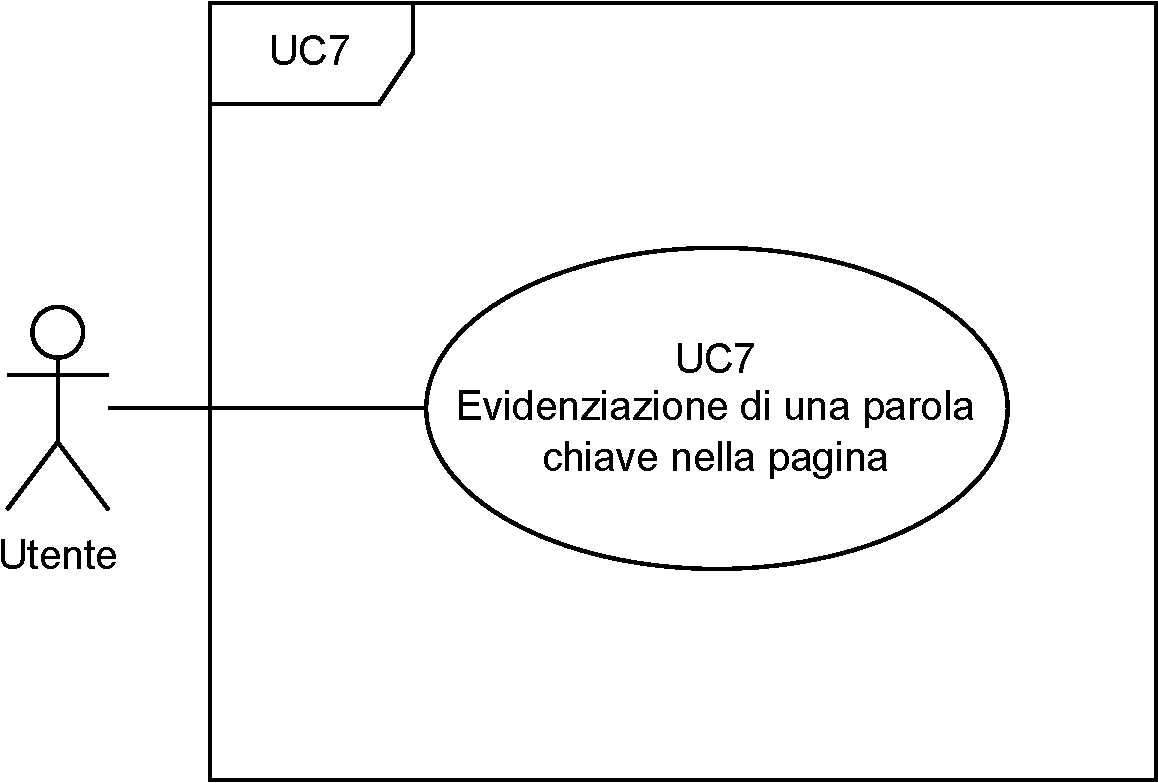
\includegraphics[width=0.6\textwidth]{usecase/uc_7.pdf}
  \caption{UC7}
  \label{fig:uc7}
\end{figure}

\begin{usecase}{8}{Visualizzazione dei risultati dell'analisi di una parola chiave}\label{UC8}
    \usecaseactors{Utente.}
    \usecasepreEnv{\begin{itemize}
        \item L'utente ha selezionato lo strumento di analisi delle parole chiave;
        \item Il sistema è attivo e funzionante.
    \end{itemize}}
    \usecasepost{L'utente visualizza i risultati dell'analisi di una parola chiave.}
    \usecaseincEnv{\begin{itemize}
        \item \hyperref[UC10]{UC10}: Visualizzazione della parola chiave vera e propria;
        \item \hyperref[UC11]{UC11}: Visualizzazione della frequenza di una parola chiave;
        \item \hyperref[UC12]{UC12}: Visualizzazione della densità di una parola chiave;
        \item \hyperref[UC13]{UC13}: Visualizzazione di una lista di tag \gls{html} rilevanti per l’analisi delle parole chiave.
    \end{itemize}}
\end{usecase}

\vspace{10pt}
\par\noindent La figura \ref{fig:uc8} illustra graficamente il caso d'uso UC8.

\begin{figure}[H]
  \centering
  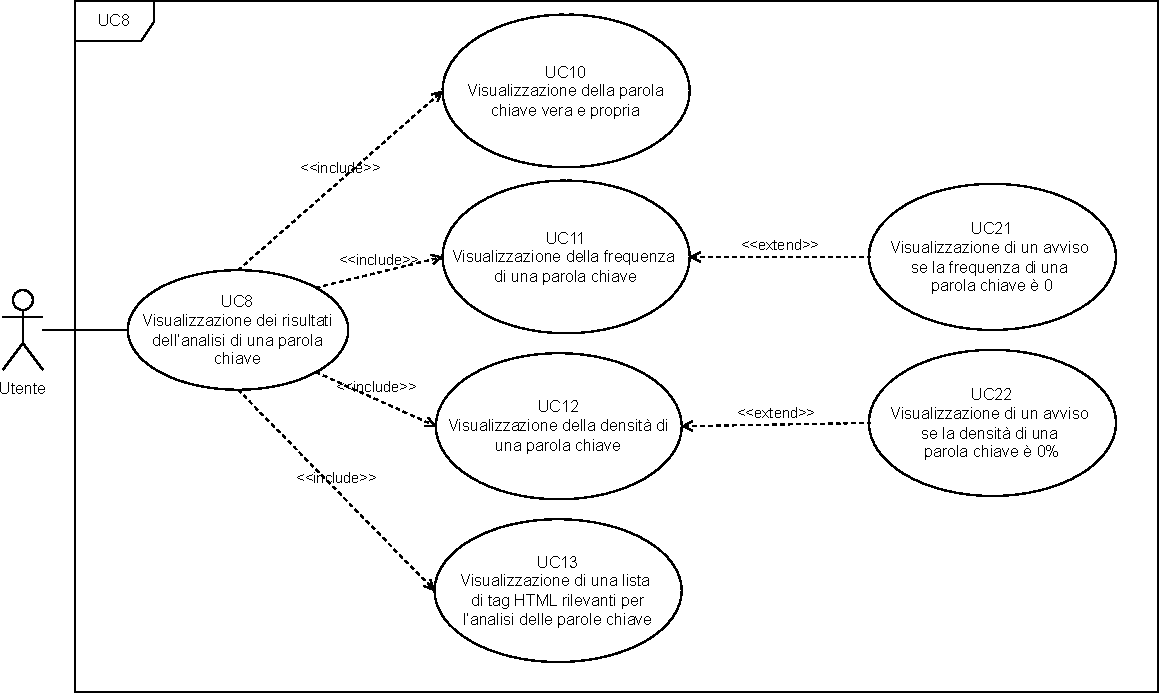
\includegraphics[width=\textwidth]{usecase/uc_8.pdf}
  \caption{UC8}
  \label{fig:uc8}
\end{figure}

\begin{usecase}{9}{Eliminazione di una parola chiave}\label{UC9}
    \usecaseactors{Utente.}
    \usecasepreEnv{\begin{itemize}
        \item L'utente ha selezionato lo strumento di analisi delle parole chiave;
        \item Il sistema è attivo e funzionante.
    \end{itemize}}
    \usecasedesc{L'utente elimina una parola chiave.}
    \usecasepost{Il sistema rimuove la parola chiave dalla lista delle keyword.}
\end{usecase}

\vspace{10pt}
\par\noindent La figura \ref{fig:uc9} illustra graficamente il caso d'uso UC9.

\begin{figure}[H]
  \centering
  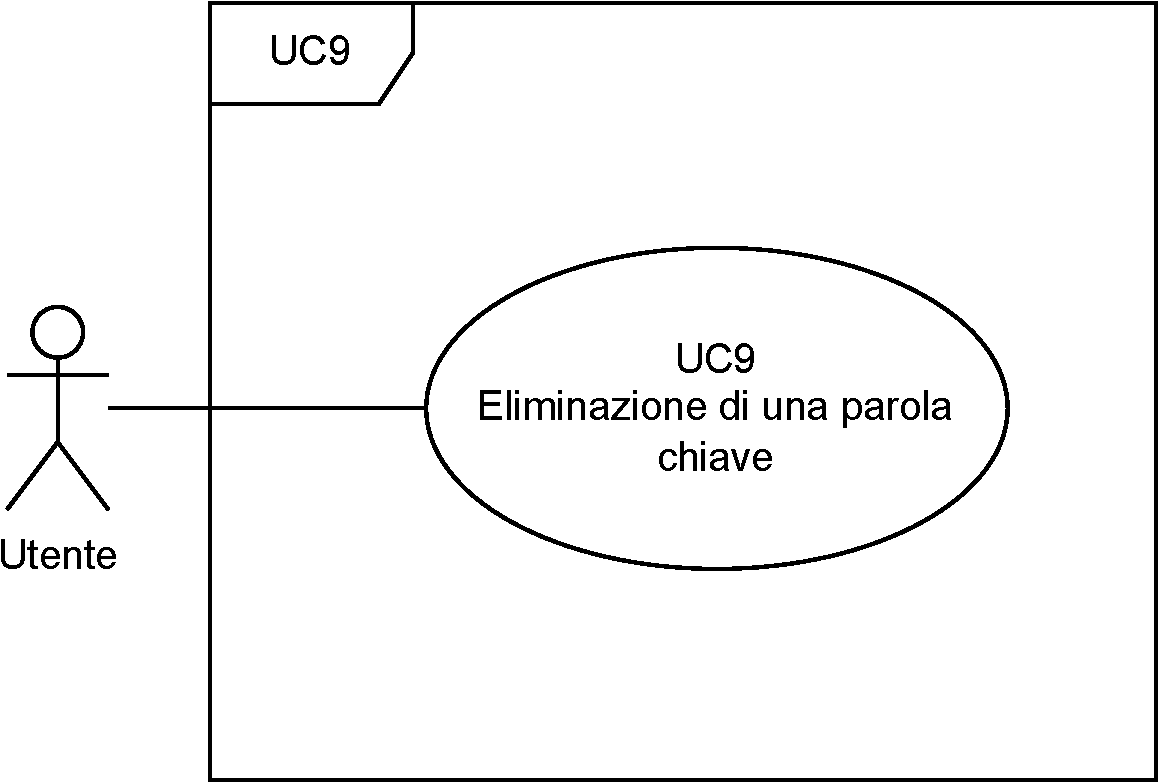
\includegraphics[width=0.6\textwidth]{usecase/uc_9.pdf}
  \caption{UC9}
  \label{fig:uc9}
\end{figure}

\begin{usecase}{10}{Visualizzazione della parola chiave vera e propria}\label{UC10}
    \usecaseactors{Utente.}
    \usecasepreEnv{\begin{itemize}
        \item L'utente ha selezionato lo strumento di analisi delle parole chiave;
        \item Il sistema è attivo e funzionante.
    \end{itemize}}
    \usecasepost{L’utente visualizza la parola chiave vera e propria (es. “JavaScript”).}
\end{usecase}

\vspace{10pt}
\par\noindent La figura \ref{fig:uc10} illustra graficamente il caso d'uso UC10.

\begin{figure}[H]
  \centering
  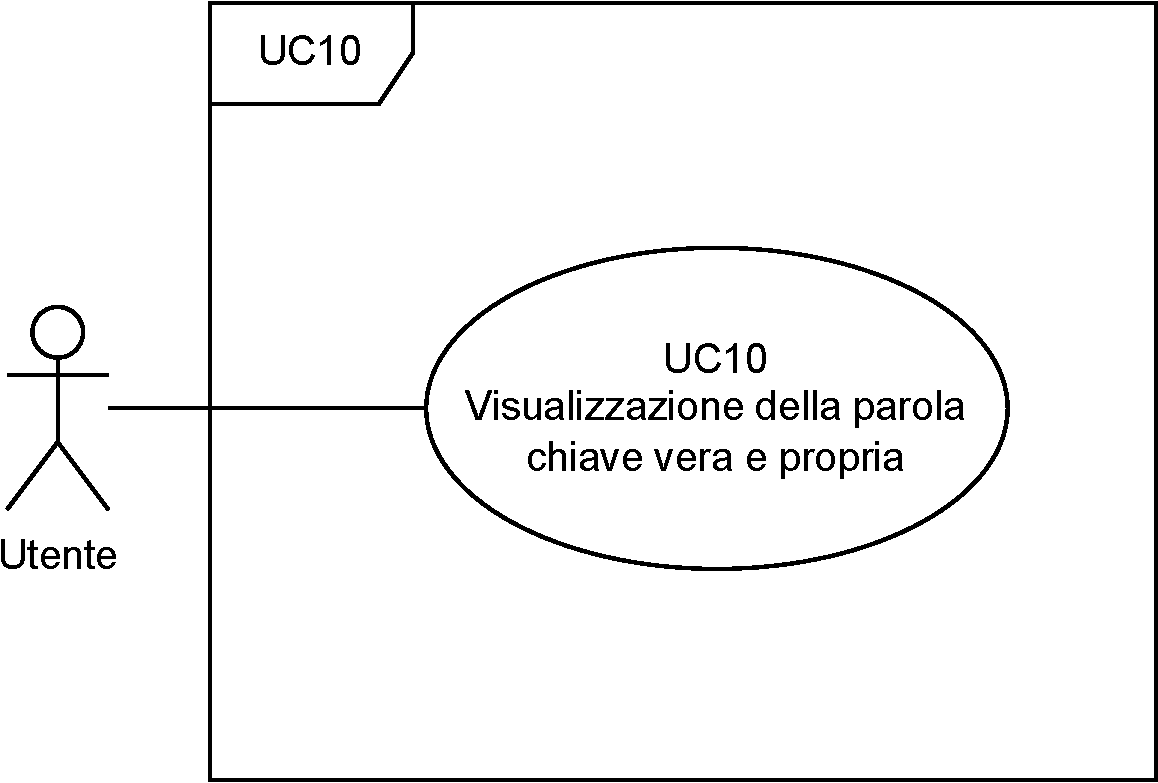
\includegraphics[width=0.6\textwidth]{usecase/uc_10.pdf}
  \caption{UC10}
  \label{fig:uc10}
\end{figure}

\begin{usecase}{11}{Visualizzazione della frequenza di una parola chiave}\label{UC11}
    \usecaseactors{Utente.}
    \usecasepreEnv{\begin{itemize}
        \item L'utente ha selezionato lo strumento di analisi delle parole chiave;
        \item Il sistema è attivo e funzionante.
    \end{itemize}}
    \usecasepost{L'utente visualizza la frequenza di una parola chiave.}
    \usecaseextEnv{\begin{itemize}
        \item \hyperref[UC19]{UC19}: Visualizzazione di un avviso se la frequenza di una parola chiave è 0.
    \end{itemize}}
\end{usecase}

\vspace{10pt}
\par\noindent La figura \ref{fig:uc11} illustra graficamente il caso d'uso UC11.

\begin{figure}[H]
  \centering
  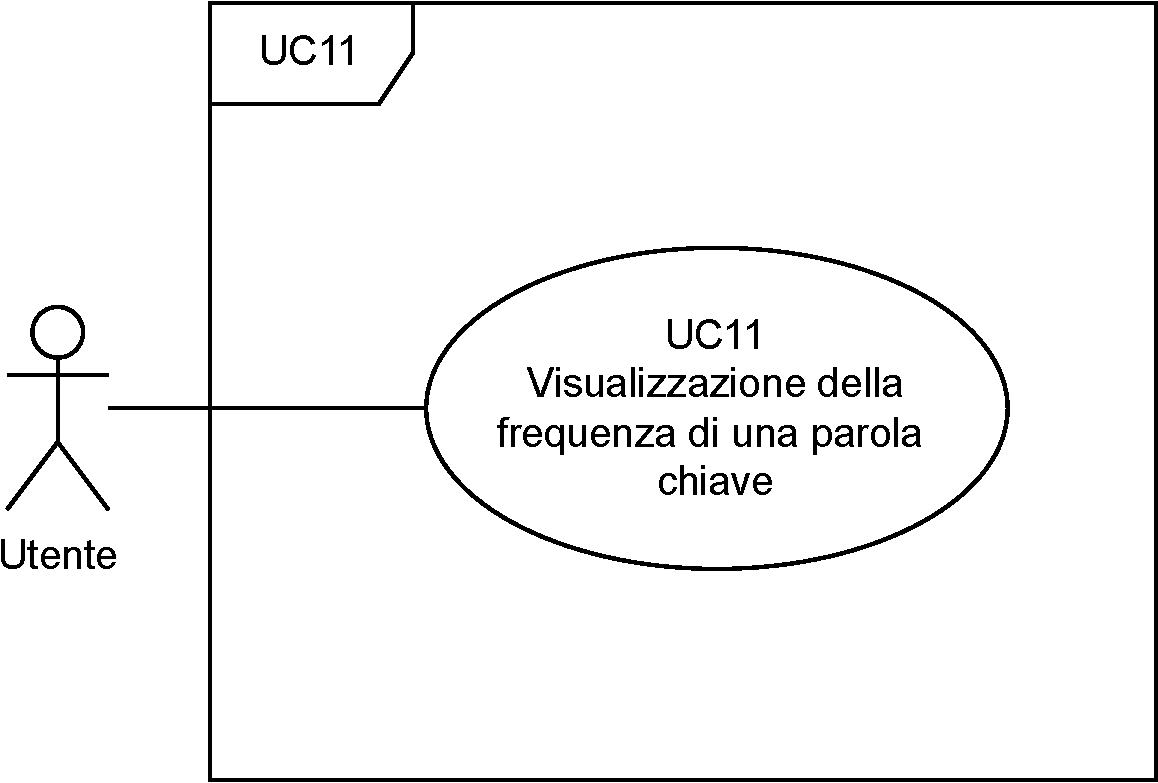
\includegraphics[width=0.6\textwidth]{usecase/uc_11.pdf}
  \caption{UC11}
  \label{fig:uc11}
\end{figure}

\begin{usecase}{12}{Visualizzazione della densità di una parola chiave}\label{UC12}
    \usecaseactors{Utente.}
    \usecasepreEnv{\begin{itemize}
        \item L'utente ha selezionato lo strumento di analisi delle parole chiave;
        \item Il sistema è attivo e funzionante.
    \end{itemize}}
    \usecasepost{L'utente visualizza la densità percentuale di una parola chiave.}
    \usecaseextEnv{\begin{itemize}
        \item \hyperref[UC20]{UC20}: Visualizzazione di un avviso se la densità di una parola chiave è 0\%.
    \end{itemize}}
\end{usecase}

\vspace{10pt}
\par\noindent La figura \ref{fig:uc12} illustra graficamente il caso d'uso UC12.

\begin{figure}[H]
  \centering
  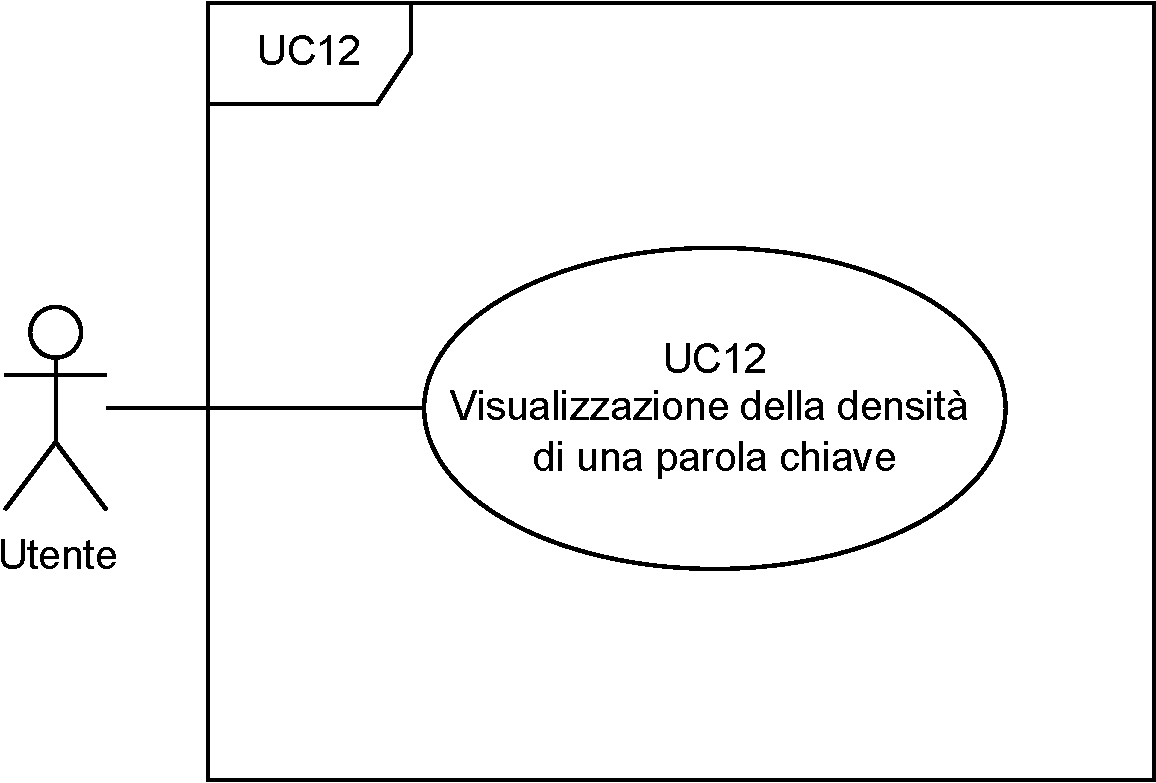
\includegraphics[width=0.6\textwidth]{usecase/uc_12.pdf}
  \caption{UC12}
  \label{fig:uc12}
\end{figure}

\begin{usecase}{13}{Visualizzazione di una lista di tag HTML rilevanti per l’analisi delle parole chiave}\label{UC13}
    \usecaseactors{Utente.}
    \usecasepreEnv{\begin{itemize}
        \item L'utente ha selezionato lo strumento di analisi delle parole chiave;
        \item Il sistema è attivo e funzionante.
    \end{itemize}}
    \usecasepost{L’utente visualizza una lista di tag \gls{html} considerati rilevanti per l’analisi delle parole chiave.}
    \usecasesubEnv{\begin{itemize}
        \item \hyperref[UC13point1]{UC13.1}: Visualizzazione di un singolo tag all’interno della lista.
    \end{itemize}}
\end{usecase}

\vspace{10pt}
\par\noindent La figura \ref{fig:uc13} illustra graficamente il caso d'uso UC13.

\begin{figure}[H]
  \centering
  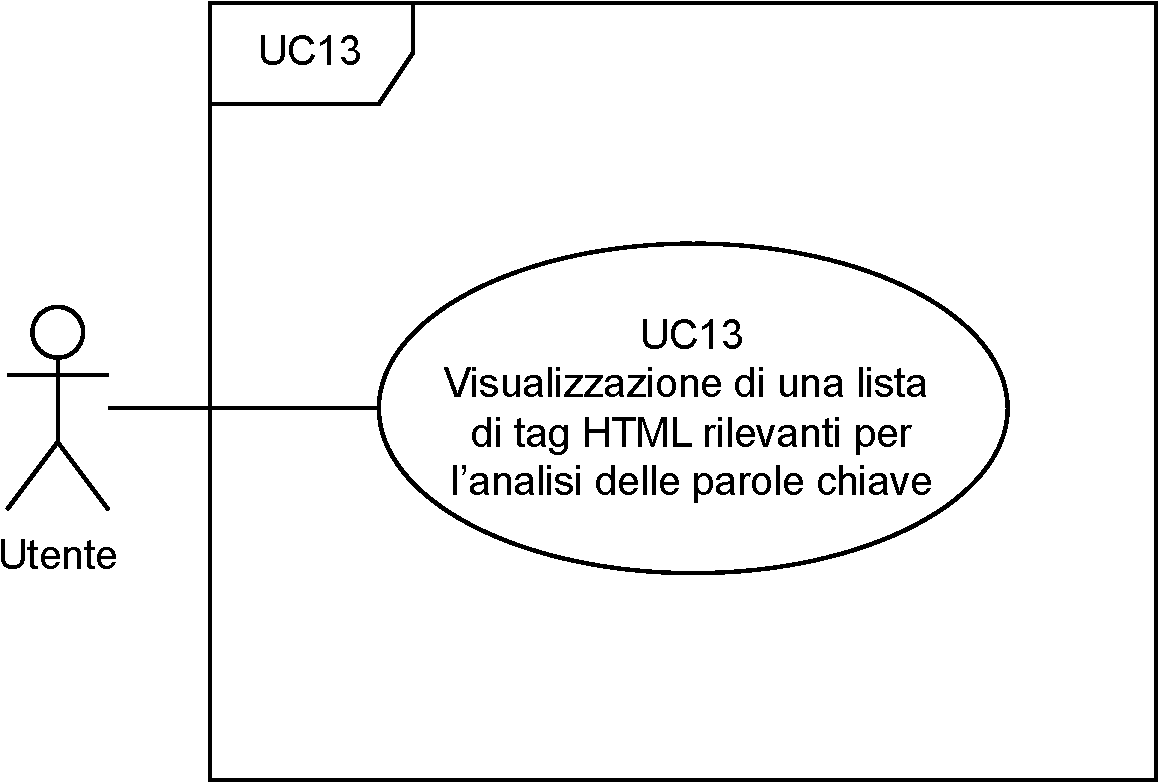
\includegraphics[width=0.6\textwidth]{usecase/uc_13.pdf}
  \caption{UC13}
  \label{fig:uc13}
\end{figure}

\begin{usecase}{13.1}{Visualizzazione di un singolo tag all’interno della lista}\label{UC13point1}
    \usecaseactors{Utente.}
    \usecasepreEnv{\begin{itemize}
        \item L'utente ha selezionato lo strumento di analisi delle parole chiave;
        \item Il sistema è attivo e funzionante;
        \item L'utente sta visualizzando i risultati dell'analisi di una parola chiave;
        \item È visibile l'elenco dei tag \gls{html}.
    \end{itemize}}
    \usecasepost{L'utente visualizza un singolo tag all’interno della lista.}
    \usecasesubEnv{\begin{itemize}
        \item \hyperref[UC13point1point1]{UC13.1.1}: Visualizzazione del nome del tag;
        \item \hyperref[UC13point1point2]{UC13.1.2}: Visualizzazione del numero di occorrenze di una parola chiave nel tag.
    \end{itemize}}
\end{usecase}

\vspace{10pt}
\par\noindent La figura \ref{fig:uc13_sottocasi} illustra graficamente i sottocasi del caso d'uso UC13.

\begin{figure}[H]
  \centering
  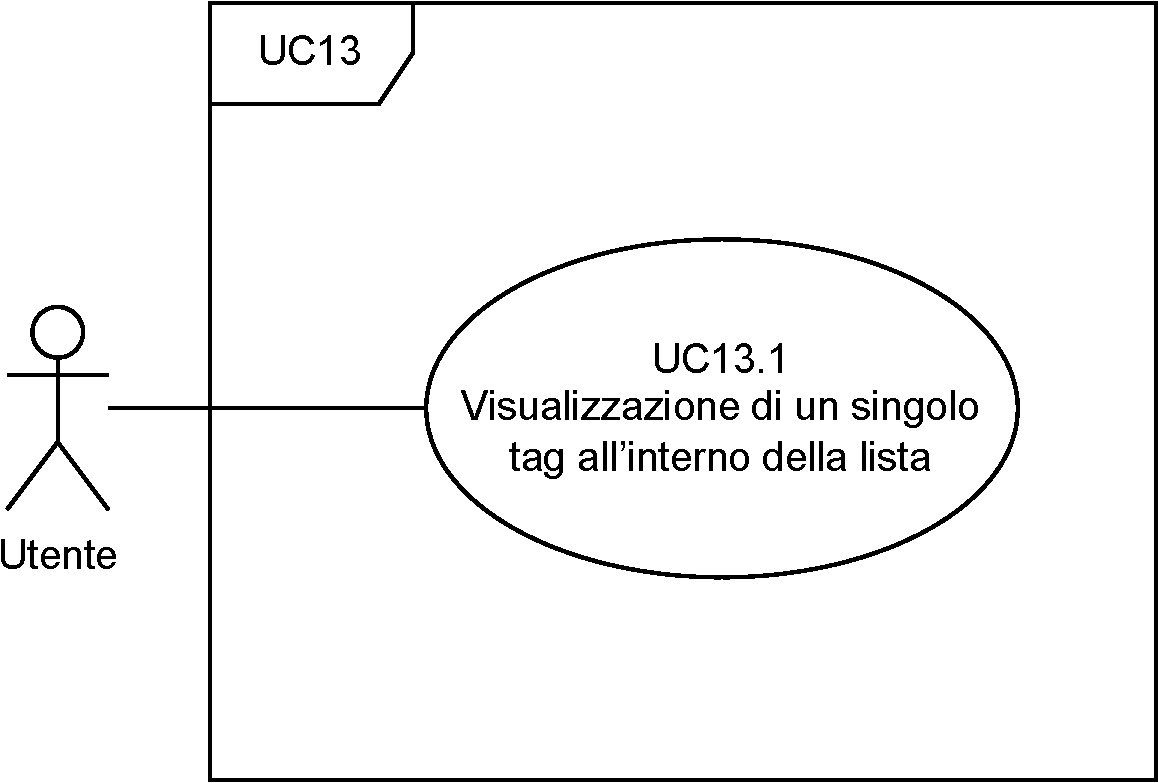
\includegraphics[width=0.6\textwidth]{usecase/uc_13_sottocasi.pdf}
  \caption{UC13 - sottocasi}
  \label{fig:uc13_sottocasi}
\end{figure}

\begin{usecase}{13.1.1}{Visualizzazione del nome del tag}\label{UC13point1point1}
    \usecaseactors{Utente.}
    \usecasepreEnv{\begin{itemize}
        \item L'utente ha selezionato lo strumento di analisi delle parole chiave;
        \item Il sistema è attivo e funzionante.
    \end{itemize}}
    \usecasepost{L'utente visualizza il nome del tag \gls{html}.}
\end{usecase}

\begin{usecase}{13.1.2}{Visualizzazione del numero di occorrenze di una parola chiave nel tag}\label{UC13point1point2}
    \usecaseactors{Utente.}
    \usecasepreEnv{\begin{itemize}
        \item L'utente ha selezionato lo strumento di analisi delle parole chiave;
        \item Il sistema è attivo e funzionante.
    \end{itemize}}
    \usecasepost{L'utente visualizza il numero di occorrenze di una parola chiave nel tag \gls{html}.}
\end{usecase}

\vspace{10pt}
\par\noindent La figura \ref{fig:uc13_1_sottocasi} illustra graficamente i sottocasi del caso d'uso UC13.1.

\begin{figure}[H]
  \centering
  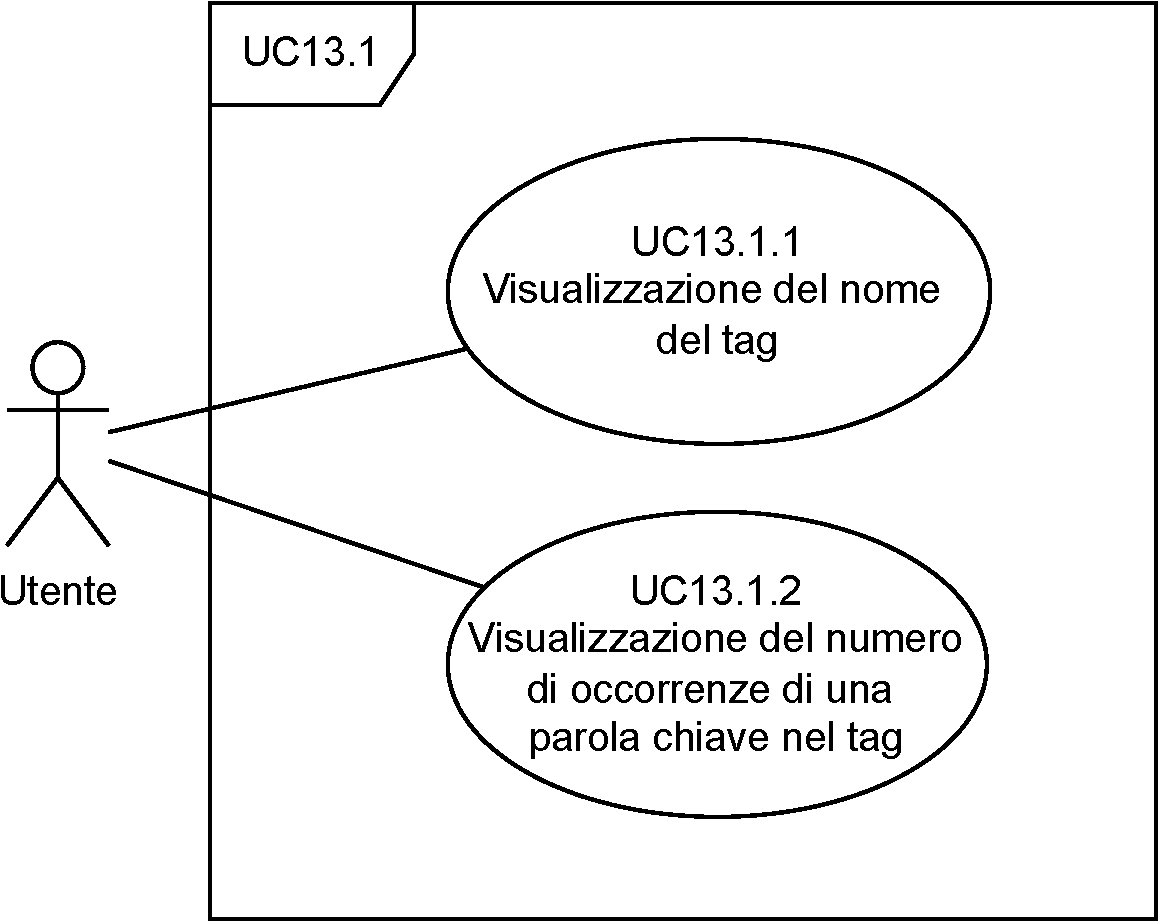
\includegraphics[width=0.6\textwidth]{usecase/uc_13_1_sottocasi.pdf}
  \caption{UC13.1 - sottocasi}
  \label{fig:uc13_1_sottocasi}
\end{figure}

\begin{usecase}{14}{Filtraggio delle parole chiave}\label{UC14}
    \usecaseactors{Utente.}
    \usecasepreEnv{\begin{itemize}
        \item L'utente ha selezionato lo strumento di analisi delle parole chiave;
        \item Il sistema è attivo e funzionante.
    \end{itemize}}
    \usecasepost{Il sistema filtra le parole chiave per nome.}
    \usecaseincEnv{\begin{itemize}
        \item \hyperref[UC3]{UC3}: Inserimento di una parola chiave.
    \end{itemize}}
\end{usecase}

\vspace{10pt}
\par\noindent La figura \ref{fig:uc14} illustra graficamente il caso d'uso UC14.

\begin{figure}[H]
  \centering
  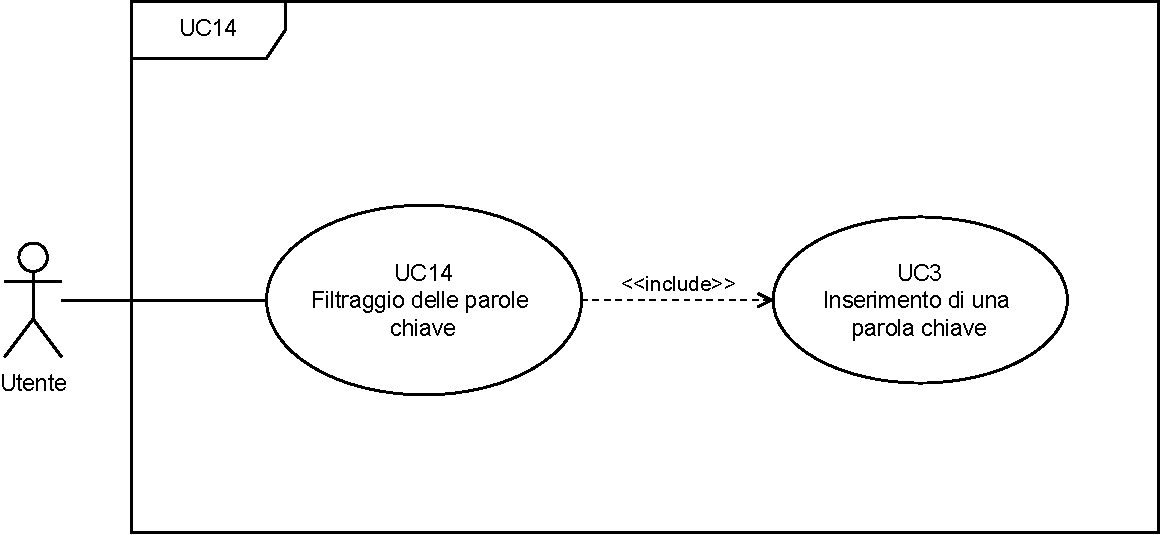
\includegraphics[width=0.95\textwidth]{usecase/uc_14.pdf}
  \caption{UC14}
  \label{fig:uc14}
\end{figure}

\begin{usecase}{15}{Ordinamento delle parole chiave}\label{UC15}
    \usecaseactors{Utente.}
    \usecasepreEnv{\begin{itemize}
        \item L'utente ha selezionato lo strumento di analisi delle parole chiave;
        \item Il sistema è attivo e funzionante.
    \end{itemize}}
    \usecasepost{Il sistema ordina le parole chiave per frequenza crescente o decrescente.}
\end{usecase}

\vspace{10pt}
\par\noindent La figura \ref{fig:uc15} illustra graficamente il caso d'uso UC15.

\begin{figure}[H]
  \centering
  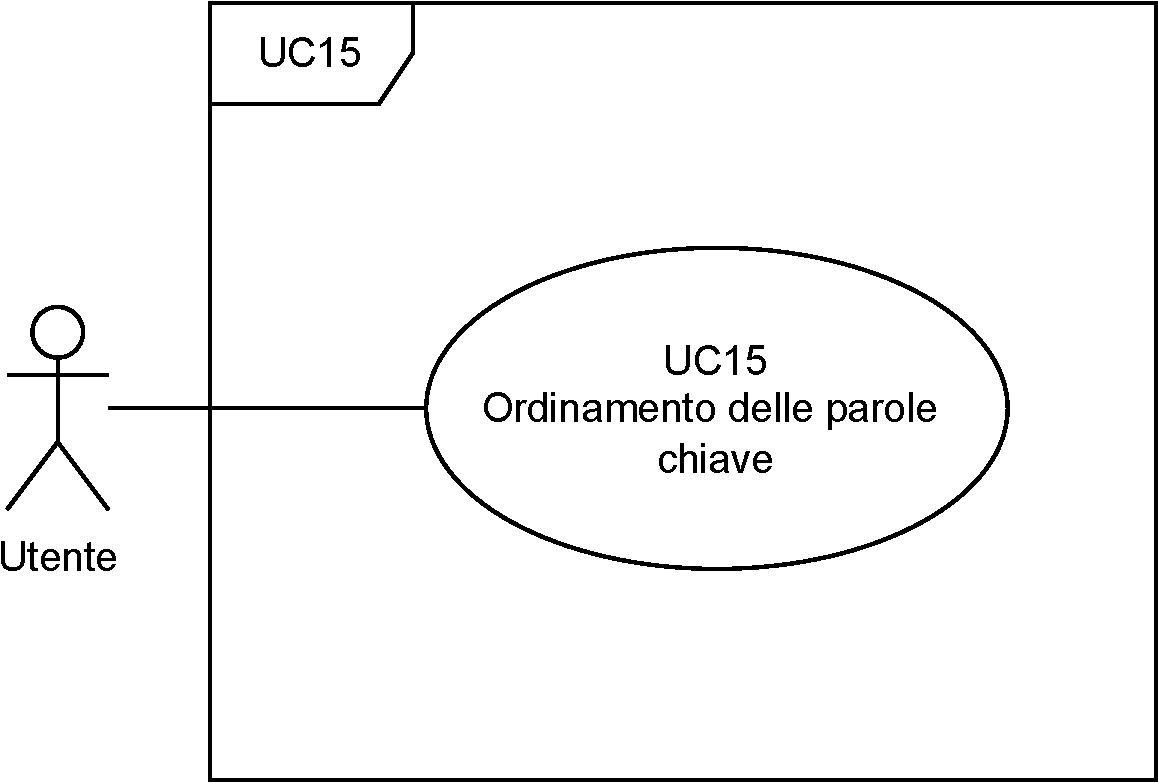
\includegraphics[width=0.6\textwidth]{usecase/uc_15.pdf}
  \caption{UC15}
  \label{fig:uc15}
\end{figure}

\begin{usecase}{16}{Rimozione dei filtri applicati}\label{UC16}
    \usecaseactors{Utente.}
    \usecasepreEnv{\begin{itemize}
        \item L'utente ha selezionato lo strumento di analisi delle parole chiave;
        \item Il sistema è attivo e funzionante.
    \end{itemize}}
    \usecasepost{L’utente rimuove i filtri applicati alle parole chiave.}
\end{usecase}

\vspace{10pt}
\par\noindent La figura \ref{fig:uc16} illustra graficamente il caso d'uso UC16.

\begin{figure}[H]
  \centering
  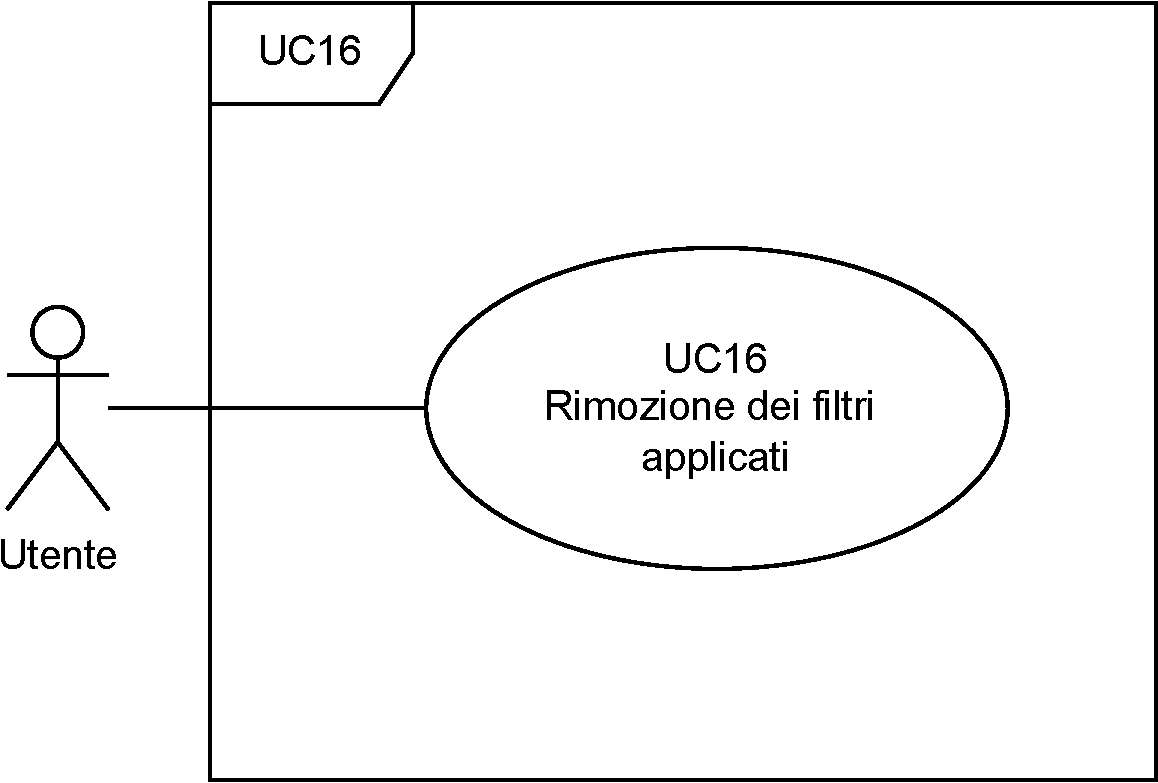
\includegraphics[width=0.6\textwidth]{usecase/uc_16.pdf}
  \caption{UC16}
  \label{fig:uc16}
\end{figure}

\begin{usecase}{17}{Navigazione delle parole chiave}\label{UC17}
    \usecaseactors{Utente.}
    \usecasepreEnv{\begin{itemize}
        \item L'utente ha selezionato lo strumento di analisi delle parole chiave;
        \item Il sistema è attivo e funzionante.
    \end{itemize}}
    \usecasepost{L’utente naviga tra le parole chiave tramite un sistema di paginazione.}
\end{usecase}

\vspace{10pt}
\par\noindent La figura \ref{fig:uc17} illustra graficamente il caso d'uso UC17.

\begin{figure}[H]
  \centering
  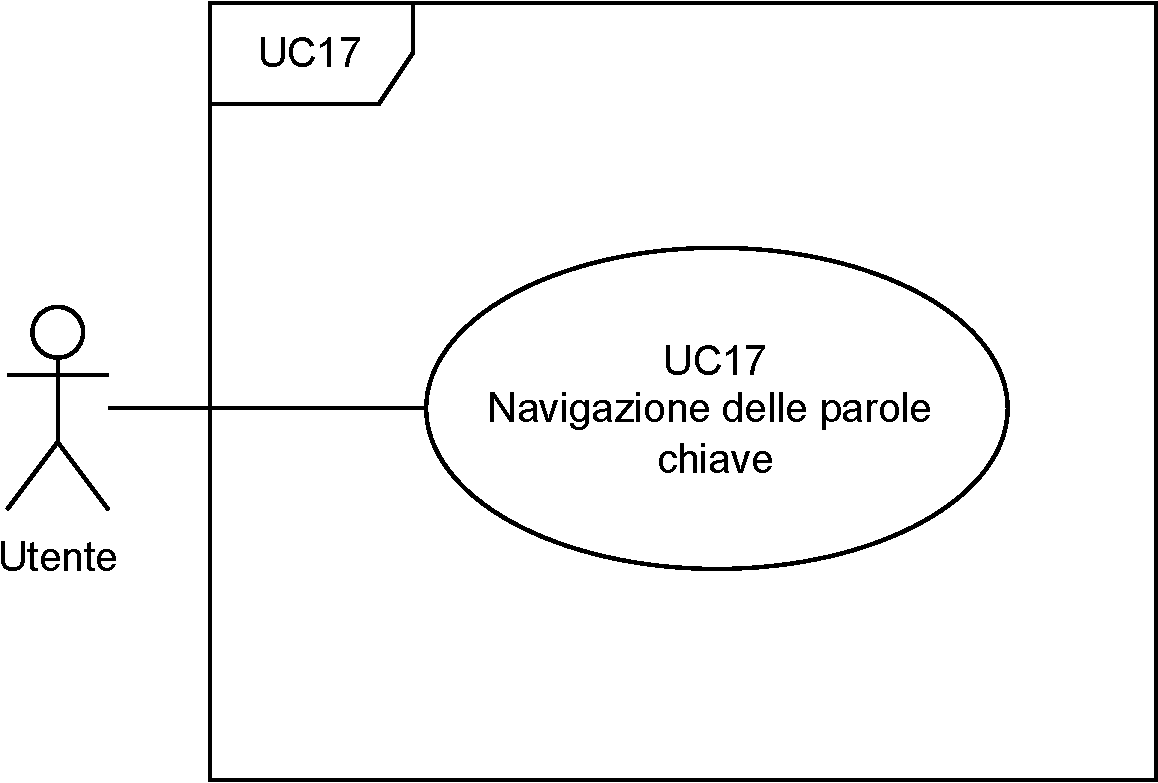
\includegraphics[width=0.6\textwidth]{usecase/uc_17.pdf}
  \caption{UC17}
  \label{fig:uc17}
\end{figure}

\begin{usecase}{18}{Aggiornamento dell'analisi delle parole chiave}\label{UC18}
    \usecaseactors{Utente.}
    \usecasepreEnv{\begin{itemize}
        \item L'utente ha selezionato lo strumento di analisi delle parole chiave;
        \item Il sistema è attivo e funzionante.
    \end{itemize}}
    \usecasedesc{L'utente aggiorna manualmente l'analisi delle parole chiave per sincronizzarla con eventuali modifiche dinamiche al \gls{dom}.}
    \usecasepost{Il sistema aggiorna l'analisi delle parole chiave.}
\end{usecase}

\vspace{10pt}
\par\noindent La figura \ref{fig:uc18} illustra graficamente il caso d'uso UC18.

\begin{figure}[H]
  \centering
  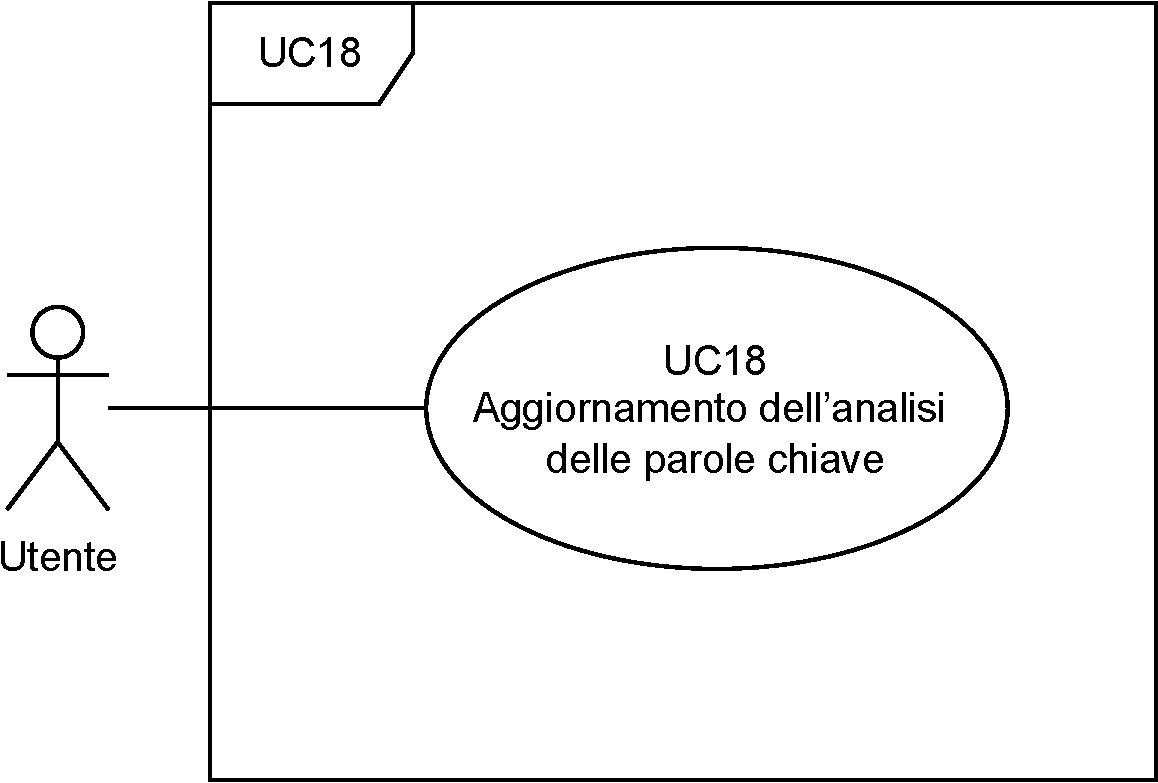
\includegraphics[width=0.6\textwidth]{usecase/uc_18.pdf}
  \caption{UC18}
  \label{fig:uc18}
\end{figure}

\begin{usecase}{19}{Visualizzazione di un avviso se il meta tag keywords non è presente}\label{UC19}
    \usecaseactors{Utente.}
    \usecasepreEnv{\begin{itemize}
        \item L'utente ha selezionato lo strumento di analisi delle parole chiave;
        \item Il sistema è attivo e funzionante;
        \item Il meta tag keywords non è presente nella pagina analizzata.
    \end{itemize}}
    \usecasepost{Il sistema mostra un avviso in cui notifica all'utente che il meta tag keywords non è presente.}
\end{usecase}

\begin{usecase}{20}{Visualizzazione di un avviso se l’attributo lang non è presente}\label{UC20}
    \usecaseactors{Utente.}
    \usecasepreEnv{\begin{itemize}
        \item L'utente ha selezionato lo strumento di analisi delle parole chiave;
        \item Il sistema è attivo e funzionante;
        \item Il tag <html> non contiene l’attributo lang.
    \end{itemize}}
    \usecasepost{Il sistema mostra un avviso in cui notifica all'utente che l'attributo lang non è presente.}
\end{usecase}

\begin{usecase}{21}{Visualizzazione di un avviso se la frequenza di una parola chiave è 0}\label{UC21}
    \usecaseactors{Utente.}
    \usecasepreEnv{\begin{itemize}
        \item L'utente ha selezionato lo strumento di analisi delle parole chiave;
        \item Il sistema è attivo e funzionante;
        \item La frequenza di una parola chiave è 0.
    \end{itemize}}
    \usecasepost{Il sistema mostra un avviso in cui notifica all'utente che la frequenza di una parola chiave è 0.}
\end{usecase}

\begin{usecase}{22}{Visualizzazione di un avviso se la densità di una parola chiave è 0\%}\label{UC22}
    \usecaseactors{Utente.}
    \usecasepreEnv{\begin{itemize}
        \item L'utente ha selezionato lo strumento di analisi delle parole chiave;
        \item Il sistema è attivo e funzionante;
        \item La densità di una parola chiave è 0\%.
    \end{itemize}}
    \usecasepost{Il sistema mostra un avviso in cui notifica all'utente che la densità di una parola chiave è 0\%.}
\end{usecase}

\begin{usecase}{23}{Aggiornamento del colore di evidenziazione per un tag HTML}\label{UC23}
    \usecaseactors{Utente.}
    \usecasepreEnv{\begin{itemize}
        \item L'utente ha selezionato lo strumento di analisi delle parole chiave;
        \item Il sistema è attivo e funzionante.
    \end{itemize}}
    \usecasepost{L'utente personalizza il colore con cui vengono evidenziate le occorrenze di una parola chiave all’interno di uno specifico tag \gls{html}.}
    \usecasesubEnv{\begin{itemize}
        \item \hyperref[UC23point1]{UC23.1}: Aggiornamento del colore di sfondo;
        \item \hyperref[UC23point2]{UC23.2}: Aggiornamento del colore del testo;
        \item \hyperref[UC23point3]{UC23.3}: Aggiornamento del colore del bordo.
    \end{itemize}}
\end{usecase}

\vspace{10pt}
\par\noindent La figura \ref{fig:uc23} illustra graficamente il caso d'uso UC23.

\begin{figure}[H]
  \centering
  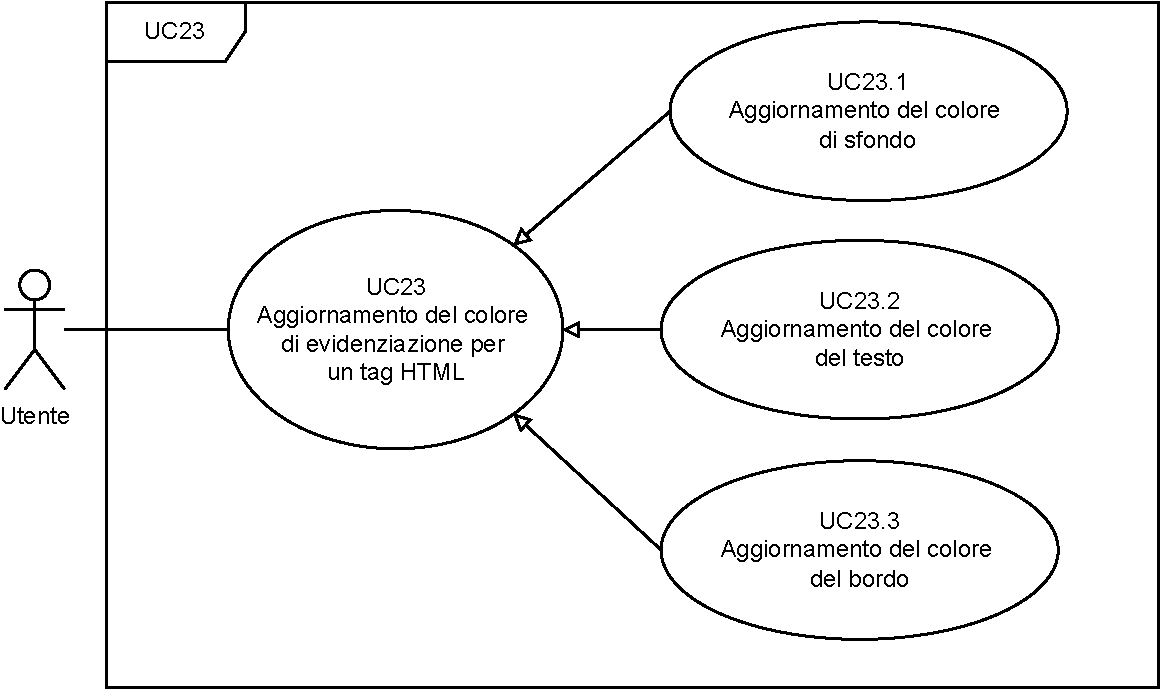
\includegraphics[width=0.95\textwidth]{usecase/uc_23.pdf}
  \caption{UC23}
  \label{fig:uc23}
\end{figure}

\begin{usecase}{23.1}{Aggiornamento del colore di sfondo}\label{UC23point1}
    \usecaseactors{Utente.}
    \usecasepreEnv{\begin{itemize}
        \item L'utente ha selezionato lo strumento di analisi delle parole chiave;
        \item Il sistema è attivo e funzionante.
    \end{itemize}}
    \usecasepost{L'utente personalizza il colore di sfondo con cui vengono evidenziate le occorrenze di una parola chiave all’interno di uno specifico tag \gls{html}.}
\end{usecase}

\begin{usecase}{23.2}{Aggiornamento del colore del testo}\label{UC23point2}
    \usecaseactors{Utente.}
    \usecasepreEnv{\begin{itemize}
        \item L'utente ha selezionato lo strumento di analisi delle parole chiave;
        \item Il sistema è attivo e funzionante.
    \end{itemize}}
    \usecasepost{L'utente personalizza il colore del testo con cui vengono evidenziate le occorrenze di una parola chiave all’interno di uno specifico tag \gls{html}.}
\end{usecase}

\begin{usecase}{23.3}{Aggiornamento del colore del bordo}\label{UC23point3}
    \usecaseactors{Utente.}
    \usecasepreEnv{\begin{itemize}
        \item L'utente ha selezionato lo strumento di analisi delle parole chiave;
        \item Il sistema è attivo e funzionante.
    \end{itemize}}
    \usecasepost{L'utente personalizza il colore del bordo con cui vengono evidenziate le occorrenze di una parola chiave all’interno di uno specifico tag \gls{html}.}
\end{usecase}

\newpage

\section{Tracciamento dei requisiti}
\par I \gls{requisiti} del progetto, individuati e formalizzati durante il processo di analisi, sono illustrati nelle tabelle \ref{tab:requisiti-funzionali}, \ref{tab:requisiti-qualitativi} e \ref{tab:requisiti-vincolo} secondo la seguente notazione:
\par \textbf{\[R[Tipologia].[Importanza].[Codice]\]} 
\par dove:
\par\vspace{20pt}
\begin{tabular}{@{}ll@{}}
    R = & requisito \\
    \textbf{Tipologia}: & \\
    \quad F = & funzionale \\
    \quad Q = & di qualità \\
    \quad V = & di vincolo/dominio \\
    \textbf{Importanza}: & \\
    \quad O = & obbligatorio \\
    \quad D = & desiderabile \\  
    \quad OP = & opzionale \\
    Codice = & codice numerico univoco \\
\end{tabular}
    
\par\vspace{30pt}

\renewcommand{\arraystretch}{1.5}
\begin{tabularx}{\textwidth}{l >{\raggedright\arraybackslash}X l}
\caption{Tabella dei requisti funzionali}
\label{tab:requisiti-funzionali} \\
\hline\hline
\textbf{Requisito} & \textbf{Descrizione} & \textbf{Fonti} \\
\endfirsthead

\caption[]{Tabella dei requisiti funzionali (continua)} \\
\hline\hline
\textbf{Requisito} & \textbf{Descrizione} & \textbf{Fonti} \\ 
\endhead

\multicolumn{3}{r}{{Continua nella prossima pagina}} \\ 
\endfoot

\hline
\endlastfoot

\hline
RF.O.1 & L'utente deve poter accedere allo strumento di analisi delle parole chiave. & \hyperref[UC1]{UC1} \\
\hline
RF.O.2 & L'utente deve poter visualizzare una panoramica dell'analisi delle parole chiave. & \hyperref[UC2]{UC2} \\
\hline
RF.O.3 & L'utente deve poter visualizzare il contenuto del meta tag keywords. & \hyperref[UC2point1]{UC2.1} \\
\hline
RF.O.4 & L'utente deve poter visualizzare il numero totale di parole nella pagina. & \hyperref[UC2point2]{UC2.2} \\
\hline
RF.D.5 & L'utente deve poter visualizzare il numero di parole uniche nella pagina. & \hyperref[UC2point3]{UC2.3} \\
\hline
RF.O.6 & L'utente deve poter visualizzare la lingua della pagina. & \hyperref[UC2point4]{UC2.4} \\
\hline
RF.O.7 & L'utente deve poter digitare una parola chiave. & \hyperref[UC3]{UC3} \\
\hline
RF.O.8 & L'utente deve poter analizzare la parola chiave digitata. & \hyperref[UC4]{UC4} \\
\hline
RF.O.9 & L'utente deve poter visualizzare una lista delle parole chiave. & \hyperref[UC5]{UC5} \\
\hline
RF.O.10 & L'utente deve poter visualizzare una lista delle parole chiave estratte dal meta tag keywords. & \hyperref[UC5point1]{UC5.1} \\
\hline
RF.O.11 & Il sistema deve visualizzare una lista delle parole chiave inserite dall'utente. & \hyperref[UC5point2]{UC5.2} \\
\hline
RF.OP.12 & L'utente deve poter visualizzare una lista delle parole chiave più frequenti. & \hyperref[UC5point3]{UC5.3} \\
\hline
RF.OP.13 & L'utente deve poter visualizzare una lista delle parole chiave più frequenti composte da un solo termine. & \hyperref[UC5point3point1]{UC5.3.1} \\
\hline
RF.OP.14 & L'utente deve poter visualizzare una lista delle parole chiave più frequenti composte da due termini. & \hyperref[UC5point3point2]{UC5.3.2} \\
\hline
RF.O.15 & L'utente deve poter visualizzare una singola parola chiave all'interno della lista. & \hyperref[UC6]{UC6} \\
\hline
RF.O.16 & Il sistema deve evidenziare tutte le occorrenze di una parola chiave nella pagina. & \hyperref[UC7]{UC7} \\
\hline
RF.O.17 & L'utente deve poter visualizzare i risultati dell'analisi di una parola chiave. & \hyperref[UC8]{UC8} \\
\hline
RF.D.18 & L'utente deve poter eliminare una parola chiave. & \hyperref[UC9]{UC9} \\
\hline
RF.O.19 & L'utente deve poter visualizzare la parola chiave vera e propria (es. “JavaScript”). & \hyperref[UC10]{UC10} \\
\hline
RF.O.20 & L'utente deve poter visualizzare la frequenza di una parola chiave. & \hyperref[UC11]{UC11} \\
\hline
RF.O.21 & L'utente deve poter visualizzare la densità di una parola chiave. & \hyperref[UC12]{UC12} \\
\hline
RF.O.22 & Il sistema deve mostrare una lista di tag \gls{html} rilevanti per l’analisi delle parole chiave. & \hyperref[UC13]{UC13} \\
\hline
RF.O.23 & L'utente deve poter visualizzare un singolo tag all'interno della lista. & \hyperref[UC13point1]{UC13.1} \\
\hline
RF.O.24 & L'utente deve poter visualizzare il nome del tag. & \hyperref[UC13point1point1]{UC13.1.1} \\
\hline
RF.O.25 & L'utente deve poter visualizzare il numero di occorrenze di una parola chiave nel tag. & \hyperref[UC13point1point2]{UC13.1.2} \\
\hline
RF.D.26 & L'utente deve poter filtrare le parole chiave per nome. & \hyperref[UC14]{UC14} \\
\hline
RF.D.27 & L'utente deve poter ordinare le parole chiave per frequenza. & \hyperref[UC15]{UC15} \\
\hline
RF.D.28 & L'utente deve poter rimuovere i filtri applicati alle parole chiave. & \hyperref[UC16]{UC16} \\
\hline
RF.O.29 & L'utente deve poter navigare tra le parole chiave tramite un sistema di paginazione. & \hyperref[UC17]{UC17} \\
\hline
RF.OP.30 & L'utente deve poter aggiornare l'analisi delle parole chiave. & \hyperref[UC18]{UC18} \\
\hline
RF.O.31 & Il sistema deve mostrare un avviso se il meta tag keywords non è presente. & \hyperref[UC19]{UC19} \\
\hline
RF.O.32 & Il sistema deve mostrare un avviso se il tag <html> non contiene l’attributo lang. & \hyperref[UC20]{UC20} \\
\hline
RF.O.33 & Il sistema deve mostrare un avviso se la frequenza di una parola chiave è 0. & \hyperref[UC21]{UC21} \\
\hline
RF.O.34 & Il sistema deve mostrare un avviso se la densità di una parola chiave è 0\%. & \hyperref[UC22]{UC22} \\
\hline
RF.OP.35 & L'utente deve poter aggiornare il colore di evidenziazione per un tag \gls{html}. & \hyperref[UC23]{UC23} \\
\hline
RF.OP.36 & L'utente deve poter personalizzare il colore di sfondo. & \hyperref[UC23point1]{UC23.1} \\
\hline
RF.OP.37 & L'utente deve poter personalizzare il colore del testo. & \hyperref[UC23point2]{UC23.2} \\
\hline
RF.OP.38 & L'utente deve poter personalizzare il colore del bordo. & \hyperref[UC23point3]{UC23.3} \\
\hline
RF.O.39 & Il sistema deve analizzare automaticamente le parole chiave specificate nel meta tag keywords. & DP\textsuperscript{*} \\
\hline
RF.OP.40 & Il sistema deve analizzare automaticamente le parole chiave più frequenti estratte dalla pagina. & DP\textsuperscript{*} \\
\hline
RF.O.41 & Il sistema deve evidenziare le parole chiave con colori diversi in base al tag \gls{html} che le racchiude. & DP\textsuperscript{*} \\
\hline
RF.OP.42 & Il sistema deve escludere le \gls{stopword} durante l'analisi del testo, in modo coerente con la lingua dichiarata nella pagina. & DP\textsuperscript{*} \\
\hline
RF.D.43 & Il sistema deve identificare le keyphrase “spezzate” su più tag \gls{html}. & DP\textsuperscript{*} \\
\end{tabularx}

\vspace{3pt}
\noindent\textsuperscript{*}~DP = Discussione con la Proponente.

\renewcommand{\arraystretch}{1.5}
\begin{tabularx}{\textwidth}{l >{\raggedright\arraybackslash}X l}
\caption{Tabella dei requisti di qualità}
\label{tab:requisiti-qualitativi} \\
\hline\hline
\textbf{Requisito} & \textbf{Descrizione} & \textbf{Fonti}\\
\endfirsthead
    
\caption[]{Tabella dei requisiti di qualità (continua)} \\
\hline\hline
\textbf{Requisito} & \textbf{Descrizione} & \textbf{Fonti} \\ 
\endhead
    
\multicolumn{3}{r}{{Continua nella prossima pagina}} \\ 
\endfoot
    
\hline
\endlastfoot

\hline
RQ.O.1 & Le funzionalità di analisi \gls{seo} devono rispettare le linee guida \gls{wcag} 2.2, livello AA. & DP\textsuperscript{*} \\
\hline
RQ.OP.2 & L'estensione deve rimanere attiva su tutte le tab. & DP\textsuperscript{*} \\
\hline
RQ.D.3 & L'utente deve poter aprire e chiudere l'estensione in modo rapido e intuitivo. & DP\textsuperscript{*} \\
\end{tabularx}

\vspace{3pt}
\noindent\textsuperscript{*}~DP = Discussione con la Proponente.

\renewcommand{\arraystretch}{1.5}
\begin{tabularx}{\textwidth}{l >{\raggedright\arraybackslash}X l}
\caption{Tabella dei requisti di vincolo/dominio}
\label{tab:requisiti-vincolo} \\
\hline\hline
\textbf{Requisito} & \textbf{Descrizione} & \textbf{Fonti}\\
\endfirsthead
        
\caption[]{Tabella dei requisiti di vincolo/dominio (continua)} \\
\hline\hline
\textbf{Requisito} & \textbf{Descrizione} & \textbf{Fonti} \\ 
\endhead
        
\multicolumn{3}{r}{{Continua nella prossima pagina}} \\ 
\endfoot
        
\hline
\endlastfoot

\hline
RV.O.1 & Lo strumento di analisi \gls{seo} deve essere reso disponibile tramite \gls{github} (come codice sorgente) o pubblicato su un'altra piattaforma ad accesso pubblico. & DP\textsuperscript{*} \\
\hline
RV.O.2 & Lo strumento di analisi \gls{seo} deve essere integrato all'interno di un'estensione per Chrome. & DP\textsuperscript{*} \\
\end{tabularx}

\vspace{3pt}
\noindent\textsuperscript{*}~DP = Discussione con la Proponente.

\par\vspace{20pt}

\subsection{Riepilogo}

\begin{table}[H]
\centering
\caption{Tabella di riepilogo dei requisiti}
\label{tab:riepilogo-requisiti}
% MAX 12.5cm
\begin{tabular}{ccccc}
\hline\hline
\textbf{Requisito} & \textbf{Obbligatorio} & \textbf{Desiderabile} & \textbf{Opzionale} & \textbf{Totale} \\ 
\hline
Funzionale & 27 & 6 & 10 & 43 \\
\hline
Di qualità & 1 & 1 & 1 & 3 \\
\hline 
Di vincolo/dominio & 2 & 0 & 0 & 2 \\
\hline
\textbf{Totale} & 30 & 7 & 11 & \textbf{48} \\ 
\hline
\end{tabular}
\end{table}

\newpage

\section{User story}

\renewcommand{\arraystretch}{1.5}
\begin{tabularx}{\textwidth}{lX}
\caption{Tabella delle user story}
\label{tab:user-story} \\
\hline\hline
\textbf{ID} & \textbf{User story}\\
\endfirsthead
    
\caption[]{Tabella delle user story (continua)} \\
\hline\hline
\textbf{ID} & \textbf{User story} \\ 
\endhead
    
\multicolumn{2}{r}{{Continua nella prossima pagina}} \\ 
\endfoot
    
\hline
\endlastfoot

\hline
1 & Come utente, voglio visualizzare una panoramica dell'analisi delle parole chiave, in modo da avere un'idea generale del contenuto della pagina. \\
\hline
2 & Come utente, voglio visualizzare il contenuto del meta tag keywords, in modo da verificare se sono state specificate delle parole chiave. \\
\hline
3 & Come utente, voglio visualizzare il numero di parole totali e uniche presenti nella pagina, in modo da valutare la qualità del contenuto. \\
\hline
4 & Come utente, voglio inserire manualmente una parola chiave, in modo da analizzare anche quelle non presenti nel meta tag keywords o non rilevate automaticamente dal sistema. \\
\hline
5 & Come utente, voglio visualizzare un elenco delle parole chiave analizzate, suddivise per categoria, in modo da facilitarne la consultazione. \\
\hline
6 & Come utente, voglio visualizzare graficamente tutte le occorrenze di una parola chiave nella pagina, con colori diversi in base al tag \gls{html} che le contiene, in modo da valutarne la distribuzione. \\
\hline
7 & Come utente, voglio visualizzare i risultati dell’analisi di una parola chiave in una sezione dedicata, in modo da potermi concentrare su una singola keyword alla volta. \\
\hline
8 & Come utente, voglio eliminare una parola chiave, in modo da mantenere pulita la lista delle keyword. \\
\hline
9 & Come utente, voglio visualizzare la frequenza e la densità di una parola chiave, in modo da capire se il suo utilizzo è eccessivo o appropriato. \\
\hline
10 & Come utente, voglio visualizzare il numero di occorrenze di una parola chiave nei principali tag \gls{html}, in modo da capire se è presente nei punti strategici della pagina. \\
\hline
11 & Come utente, voglio filtrare le parole chiave per nome, in modo da individuare più facilmente quelle di mio interesse. \\
\hline
12 & Come utente, voglio ordinare le parole chiave per frequenza, in modo da semplificare l’accesso a quelle più o meno ricorrenti. \\
\hline
13 & Come utente, voglio rimuovere i filtri applicati, in modo da ripristinare la lista delle parole chiave. \\
\hline
14 & Come utente, voglio navigare tra le parole chiave mediante un sistema di paginazione, in modo da scorrere facilmente l’intera lista. \\
\hline
15 & Come utente, voglio aggiornare l'analisi delle parole chiave, in modo da sincronizzarla con eventuali modifiche dinamiche al \gls{dom}. \\
\hline
16 & Come utente, voglio personalizzare i colori di sfondo, testo e bordo associati a un tag \gls{html}, in modo da adattare l'evidenziazione delle parole chiave alle mie esigenze visive. \\
\hline
17 & Come utente, voglio analizzare anche le parole chiave “spezzate” su più tag \gls{html}, in modo da gestire correttamente le keyphrase. \\
\hline
18 & Come utente, voglio che lo strumento di analisi \gls{seo} sia accessibile a tutti. \\
\end{tabularx}